%%%%%%%%%%%%%%%%%%%%%%%%%%%%%%%%%%%%%%%%%%%%%%%%%%%%%%%%%%%%%%%%%%%%%%%%%%%%%%%%
% ISE Lab -- Topic
% Giovanni Ciatto
% Alma Mater Studiorum - Università di Bologna
% mailto:giovanni.ciatto@unibo.it
%%%%%%%%%%%%%%%%%%%%%%%%%%%%%%%%%%%%%%%%%%%%%%%%%%%%%%%%%%%%%%%%%%%%%%%%%%%%%%%%
%\documentclass[handout]{beamer}\mode<handout>{\usetheme{default}}
%
\documentclass[presentation]{beamer}\mode<presentation>{\usetheme{AMSBolognaFC}}
%\documentclass[handout]{beamer}\mode<handout>{\usetheme{AMSBolognaFC}}
%%%%%%%%%%%%%%%%%%%%%%%%%%%%%%%%%%%%%%%%%%%%%%%%%%%%%%%%%%%%%%%%%%%%%%%%%%%%%%%%
\usepackage{ise-lab-common}
\usepackage{ise-lab-perception-actuation}
% version
\newcommand{\versionmajor}{1}
\newcommand{\versionminor}{0}
\newcommand{\versionpatch}{0}
\newcommand{\version}{\versionmajor.\versionminor.\versionpatch}
%%%%%%%%%%%%%%%%%%%%%%%%%%%%%%%%%%%%%%%%%%%%%%%%%%%%%%%%%%%%%%%%%%%%%%%%%%%%%%%%
\title[\currentLab{} -- Perception \& Actuation]{Perception \& Actuation from the Agent Perspective}
%
\subtitle{\courseName{} / Module \moduleN{} (\courseAcronym)}
%
\author[\sspeaker{\gcShort}]{\speaker{\gcFull} \\ \gcEmail}
%
\institute[\disiShort, \uniboShort]{\disi{} (\disiShort)\\\unibo}
%
\date[A.Y. \academicYear{} (v.\ \version)]{Academic Year \academicYear{}\\(version \version)}
%
%%%%%%%%%%%%%%%%%%%%%%%%%%%%%%%%%%%%%%%%%%%%%%%%%%%%%%%%%%%%%%%%%%%%%%%%%%%%%%%%
\begin{document}
%%%%%%%%%%%%%%%%%%%%%%%%%%%%%%%%%%%%%%%%%%%%%%%%%%%%%%%%%%%%%%%%%%%%%%%%%%%%%%%%

%/////////
\frame{\titlepage}
%/////////

%%===============================================================================
\section*{Outline}
%%===============================================================================
%
%%/////////
\frame[c]{\tableofcontents[hideallsubsections]}
%%/////////

%===============================================================================
\section{Premises}
%===============================================================================

\begin{frame}{Lecture Goals}
    \begin{itemize}
        \item Understand how to enable the perception and actuation from the agent perspective
        \item Understand the notion of layered software system
        \item Understand the key role of Application Programming Interfaces (API)
    \end{itemize}
\end{frame}

%===============================================================================
\section{(Software) Environments}
%===============================================================================

\begin{frame}{The Role of Perception and Actuation}
    \begin{block}{\textbf{Environment} = anything laying outside the \textbf{agents}}
        \begin{itemize}
            \item
              Can be \alert{perceived} via \emph{sensors}
            \item
              Can be \alert{affected} via \emph{actuators}
        \end{itemize}
    \end{block}

    \begin{center}
        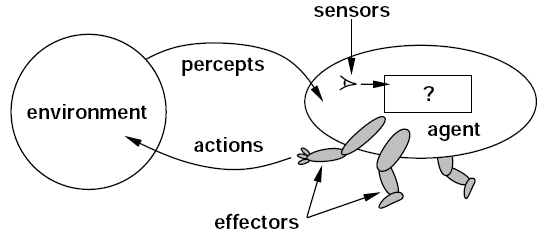
\includegraphics[width=.5\linewidth]{figures/agent-environment.png}
    \end{center}

    \begin{alertblock}{About \textbf{computational} agents}
        \begin{itemize}
            \item `Perception' $\approx$ \alert{input}
            \item `Actuation' $\approx$ \alert{output}
        \end{itemize}
    \end{alertblock}
\end{frame}

\begin{frame}{Layered View of the Software Agent}
    Software agents can be abstractly modelled as composed by \alert{layers}:
    %
    \begin{columns}
        \begin{column}{.5\linewidth}
            \begin{enumerate}
                \item Some control software
                %
                \begin{itemize}
                    \item[eg] Java / logic / AgentSpeak program
                \end{itemize}
                
                \item Some interpreter for that software (e.g.~JVM, Prolog interpreter, Jason)
                %
                \begin{itemize}
                    \item[eg] Java / logic interpreter, Jason
                \end{itemize}

                \item Some OS mediating the usage of HW resources for the interpreter
                
                \item Hardware resources
                %
                \begin{itemize}
                    \item[eg] memory, storage, computational power, I/O (there including networking)
                \end{itemize}
            \end{enumerate}
        \end{column}
        \begin{column}{.5\linewidth}
            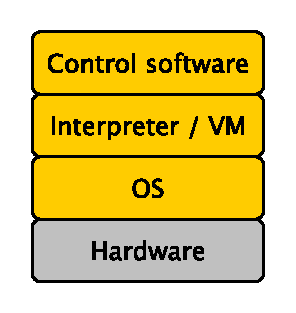
\includegraphics[width=\linewidth]{figures/layers.pdf}
        \end{column}
    \end{columns}
\end{frame}

\begin{frame}[allowframebreaks]{Actions from the Agent Perspective}
    \begin{itemize}
        \item The environment is shaped by what perceptual/actuatory actions agents can perform
        %
        \begin{itemize}
            \item[eg] sensing enviromental properties (temperature, humidity, light, etc.)
            \item[eg] sensing distances, obstacles, etc.
            \item[eg] moving wheels or harms, sucking or pushing air, etc. 
        \end{itemize}

        \bigskip

        \item The agent may also be endowed with \alert{epistemic} capabilities
        %
        \begin{itemize}
            \item[eg] memorise new knowledge
            \item[eg] forget (or update) memorised knowledge
        \end{itemize}
    \end{itemize}

    \framebreak

    \begin{alertblock}{Actions may \textbf{fail} (in so many ways!)}
        \begin{itemize}
            \item[a.] perceptual actions may provide \alert{imprecise} or \alert{meaningless} percept
            %
            \begin{itemize}
                \item[b.] or fail in providing a percept at all
            \end{itemize}

            \item[c.] actuatory actions may \alert{silently} fail by \alert{provoking no effect}
            %
            \begin{itemize}
                \item[d.] or explicitly fail returning some feedback to the agent
            \end{itemize}
        \end{itemize}        
    \end{alertblock}
    %
    \begin{itemize}
        \item situations \alert{a.} and \alert{c.} are very subtle to spot
        %
        \begin{itemize}
            \item since they're undistinguishable from `correct' actions
        \end{itemize}

        \item situations \alert{b.} and \alert{d.} subtend some form of \alert{proprioception}
    \end{itemize}
\end{frame}

\begin{frame}[allowframebreaks]{Actions from the \textbf{Software} Agent Perspective}

    \begin{alertblock}{Endowing agents with some perceptual/actuatory action requires}
        \begin{enumerate}
            \item some enabling HW facility to be present
            \item some OS functionality enabling the usage of that HW facility
            \item the interpreter to know how to call that OS functionality
            \item the programming language to have some ad-hoc API wrapping the OS functionality
        \end{enumerate}
    \end{alertblock}

    \begin{exampleblock}{The file system as an environment}
        \begin{itemize}
            \item \alert{reading} a file as a string, given its path as the \alert{perception} action
            %
            \begin{itemize}
                \item fails explicitly  when the path is missing, or non-readable
            \end{itemize}

            \item \alert{writing} a file as a string, given its path as the \alert{actuation} action
            %
            \begin{itemize}
                \item fails when the path is missing, or non-readable
            \end{itemize}
        \end{itemize}
    \end{exampleblock}
\end{frame}

\section{Logic Agents}

\begin{frame}[allowframebreaks]{Logic Agents}
    \begin{block}{Goal-\textbf{driven} logic solvers are (simple) \textbf{reasoning} agents}
        \begin{itemize}
            \item Knowledge base $\rightarrow$ memory
            \item Resolution $\rightarrow$ thinking / reasoning
            \item Assertion/retraction $\rightarrow$ epistemic actions
            \item ??? $\rightarrow$ Actuation
            \item ??? $\rightarrow$ Perception
            \item ??? $\rightarrow$ Environment
        \end{itemize}
    \end{block}

    \framebreak

    Basic stub of Prolog agent:
    %
    \prologimport{listings/logic-agent-stub.pl}
    %
    which is the same as:
    %
    \prologimport{listings/logic-agent-stub2.pl}

    \begin{block}{Goal-\textbf{driven} logic solvers are (simple) \textbf{reasoning} agents}
        \begin{itemize}
            \item Knowledge base $\rightarrow$ memory
            \item Resolution $\rightarrow$ thinking / reasoning
            \item Assertion/retraction $\rightarrow$ epistemic actions
            \item \alert{Write $\rightarrow$ Actuation}
            \item ??? $\rightarrow$ Perception
            \item ??? $\rightarrow$ Environment
        \end{itemize}
    \end{block}
\end{frame}

\begin{frame}[allowframebreaks]{Example -- Thermostat agent (maintenance)}

    \prologimport[basicstyle=\tiny\ttfamily]{listings/thermostat-agent.pl}

    \framebreak

    \begin{exampleblock}{Goal}
        \begin{itemize}
            \item \alert{maintain} the temperature into the \alert{warm} range
        \end{itemize}
    \end{exampleblock}

    \begin{alertblock}{Remarks}
        \begin{itemize}
            \item Knowledge base $\rightarrow$ memory
            \item Resolution $\rightarrow$ thinking / reasoning
            \item Assertion/retraction $\rightarrow$ epistemic actions
            \item \alert{Write file $\rightarrow$ Actuation}
            \item \alert{Read file $\rightarrow$ Perception}
            \item \alert{File system $\rightarrow$ Environment}
        \end{itemize}
    \end{alertblock}

    \begin{block}{Required functionalities}
        \begin{enumerate}    
            \item reading a file as a string, given its path as the perception action
            %
            \begin{itemize}
                \item \pl{read\_text/2} \alert{(to be implemented)}
            \end{itemize}

            \item writing a file as a string, given its path as the actuation action
            %
            \begin{itemize}
                \item \pl{write\_text/2} \alert{(to be implemented)}
            \end{itemize}

            % \item capability to memorize custom information
            % %
            % \begin{itemize}
            %     \item \pl{assert/1}, \pl{asserta/1}, \pl{assertz/1} \alert{(provided by standard Prolog)}
            % \end{itemize}

            % \item capability to discard memorised information
            % %
            % \begin{itemize}
            %     \item \pl{retract/1} \alert{(provided by standard Prolog)}
            % \end{itemize}
        \end{enumerate}
    \end{block}
\end{frame}

\begin{frame}[allowframebreaks]{Example -- Thermostat agent (achievement)}
\label{slide:achievement}

    \prologimport[basicstyle=\tiny\ttfamily]{listings/thermostat-agent2.pl}

    \framebreak

    \begin{exampleblock}{Goal}
        \begin{itemize}
            \item \alert{achieve} a situation where temperature is into the \alert{warm} range
            %
            \begin{itemize}
                \item[!] then stop
            \end{itemize}
        \end{itemize}
    \end{exampleblock}

    \begin{block}{How to realise these kind of functionalities?}
        \begin{enumerate}    
            \item reading a file as a string, given its path as the perception action
            %
            \begin{itemize}
                \item \pl{read\_text/2} \alert{(to be implemented)}
            \end{itemize}

            \item writing a file as a string, given its path as the actuation action
            %
            \begin{itemize}
                \item \pl{write\_text/2} \alert{(to be implemented)}
            \end{itemize}

            \item capability to memorize custom information
            %
            \begin{itemize}
                \item \pl{assert/1}, \pl{asserta/1}, \pl{assertz/1} \alert{(provided by standard Prolog)}
            \end{itemize}

            \item capability to discard memorised information
            %
            \begin{itemize}
                \item \pl{retract/1} \alert{(provided by standard Prolog)}
            \end{itemize}
        \end{enumerate}
    \end{block}
\end{frame}

\begin{frame}[allowframebreaks]{Example -- Thermostat agent}
    \begin{block}{Questions}
        \begin{enumerate}
            \item Is the thermostat agent \alert{pro-active} or \alert{re-active}?
            
            \item Is the thermostat agent \alert{autonomous}?
            %
            \begin{itemize}
                \item w.r.t. \alert{motivational} autonomy?
                \item w.r.t. \alert{executive} autonomy?
                \item w.r.t. \alert{computational} autonomy?
            \end{itemize}

            \item Is the thermostat agent relying on a \alert{strong} or \alert{weak} notion of `goal'?
        \end{enumerate}
    \end{block}

    \framebreak

    \begin{block}{Open problems}
        \begin{itemize}
            \item How to endow logic agents with new \alert{actions}?
            %
            \begin{itemize}
                \item[ie] how to realise the \alert{\pl{read\_text/2}} and \alert{\pl{write\_text/2}} functionalities?
            \end{itemize}

            \medskip

            \item We need some mechanism to extend of the logic language API\ldots
            %
            \begin{itemize}
                \item \ldots possibly, supporting the exploitation of OS resources
    
                \item \ldots possibly, supporting the generation of side effects into the solver
            \end{itemize}
        \end{itemize}
    \end{block}
    %
    \begin{itemize}
        \item[cf.] exercises on slide \ref{slide:exercies} 
    \end{itemize}
\end{frame}

%===============================================================================
\section{Generators}
%===============================================================================

\begin{frame}[allowframebreaks]{The notion of `Generator'\ccite{2pkt-jelia2021}}
    \begin{center}
        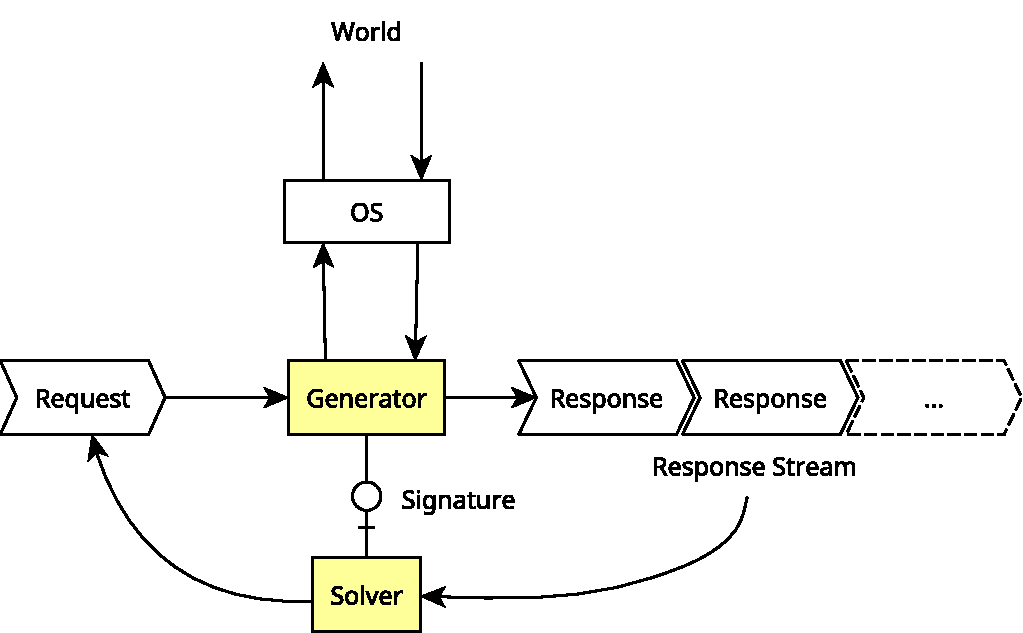
\includegraphics[width=.7\linewidth]{figures/generator.pdf}
    \end{center}

    \begin{block}{Informal definition}
        \begin{itemize}
            \item Servers serving a solver's requests to perform actions
            %
            \begin{itemize}
                \item providing 1, or more responses
            \end{itemize}
            \item A particular case of \alert{artefact}, under a MAS perspective
        \end{itemize}
    \end{block}

    \begin{block}{Defitinion}
        \begin{description}
            \item[Signature:] name + arity ($\approx$ logic API)
            \item[Behaviour:] function mapping \alert{requests} to \alert{\emph{streams} of responses}
            \item[Requests:] carry information about
            %
            \begin{itemize}
                \item the execution context (at the time of request issuing)
                \item the \emph{actual} arguments of the request
            \end{itemize}
            \item[Responses:] carry information about
            %
            \begin{itemize}
                \item success, failure, or errors
                \item substitutions to be applied to resolution
                \item side effects to be applied to the execution context
            \end{itemize}
        \end{description}
    \end{block}

    \begin{block}{Workflow}
        \begin{enumerate}\small
            \item While solving a (sub-)goal the solver may \alert{select} a generator
            %
            \begin{itemize}\scriptsize
                \item by its \alert{signature}
            \end{itemize}

            \item Then, the solver creates a \alert{request} to be sent to the generator
            
            \item The generator is then triggered: it produces a \alert{stream of responses} 
            
            \item The solver \alert{lazily consumes} the stream of responses
            %
            \begin{itemize}\scriptsize
                \item \alert{when} a response is consumed depends on \alert{how} the solver performs resolution
                \item consuming a response implies \alert{reifying} the side effects it is carrying
            \end{itemize}
            
            \item Each response constitutes a \alert{branch} in the proof three, \alert{to be explored}
            %
            \begin{itemize}\scriptsize
                \item[eg] via \alert{backtracking} 
            \end{itemize}
        \end{enumerate}
    \end{block}

    \begin{center}
        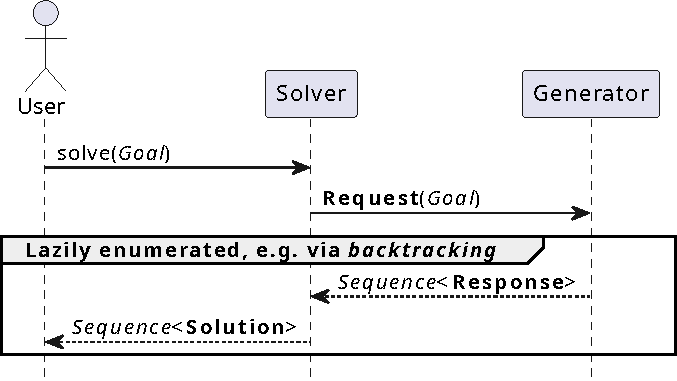
\includegraphics[width=.8\linewidth]{figures/primitive-usage.pdf}
    \end{center}
\end{frame}

\begin{frame}[allowframebreaks]{The notion of `\kt{Primitive}' in \twopkt{}}
    \begin{itemize}
        \item Generators are realised via by the \kt{Primitive} type hierarchy in \twopkt{}
        %
        \begin{center}
            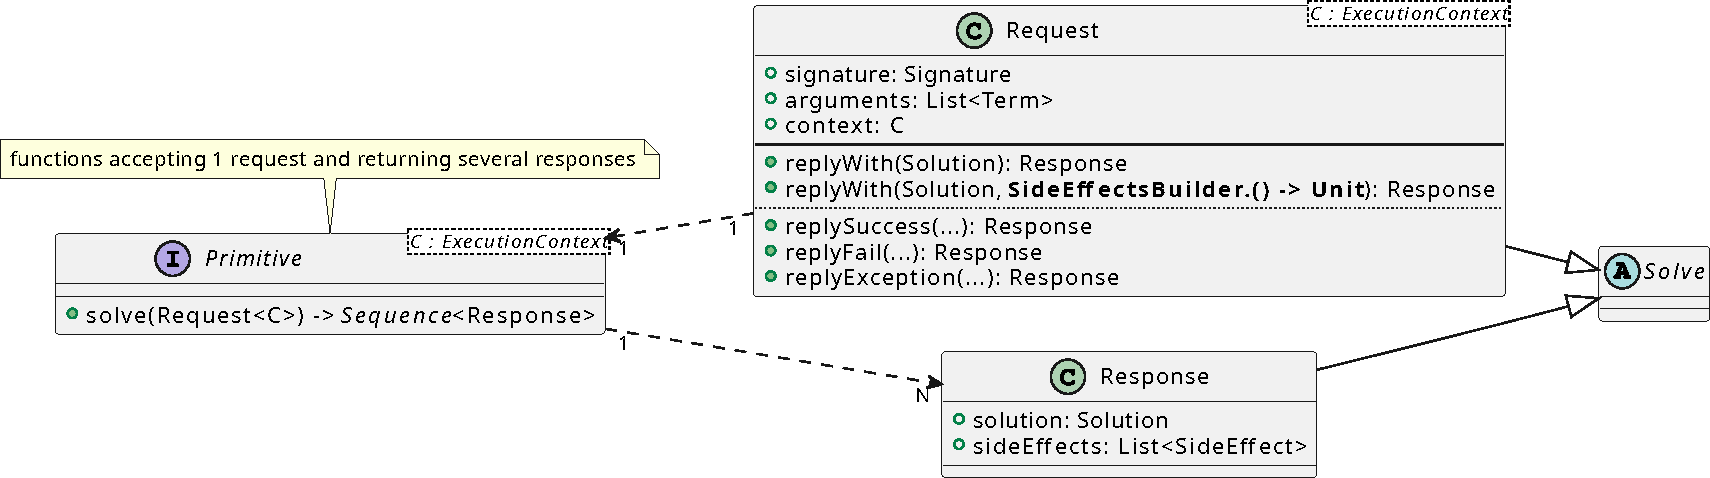
\includegraphics[width=.5\linewidth]{figures/primitive.pdf}
        \end{center}
        %
        \begin{itemize}
            \item as well as by the \kt{Solve.Request} and \kt{Solve.Response} types
        \end{itemize}

        \framebreak

        \item Upon creation, solver accept \kt{Libraries}, containing zero or more primitives
        %
        \begin{itemize}
            \item standard built-ins are constructed in this way
        \end{itemize}

        \bigskip

        \item During resolution, solvers may exploit primitives to solve (sub-)goals 
        
        \bigskip

        \item Primitives take precedence over ordinary logic rules
    \end{itemize}
\end{frame}

\begin{frame}{\kt{Primitive}s in \twopkt{} -- Example: \pl{natural/1}}
    \kotlinimport[basicstyle=\tiny\ttfamily]{listings/NatPrimitive.kt}
\end{frame}

\begin{frame}[allowframebreaks]{In practice, one may exploit \kt{PrimitiveWrapper}s}
    \begin{block}{The \kt{PrimitiveWrapper} type hierarchy}
        A pool of abstract classes factorising common aspects of primitives' implementation
        %
        \begin{itemize}
            \item primitive wrapper $\approx$ signature + primitive + utility methods
        \end{itemize}
    \end{block}

    \framebreak

    \begin{center}
        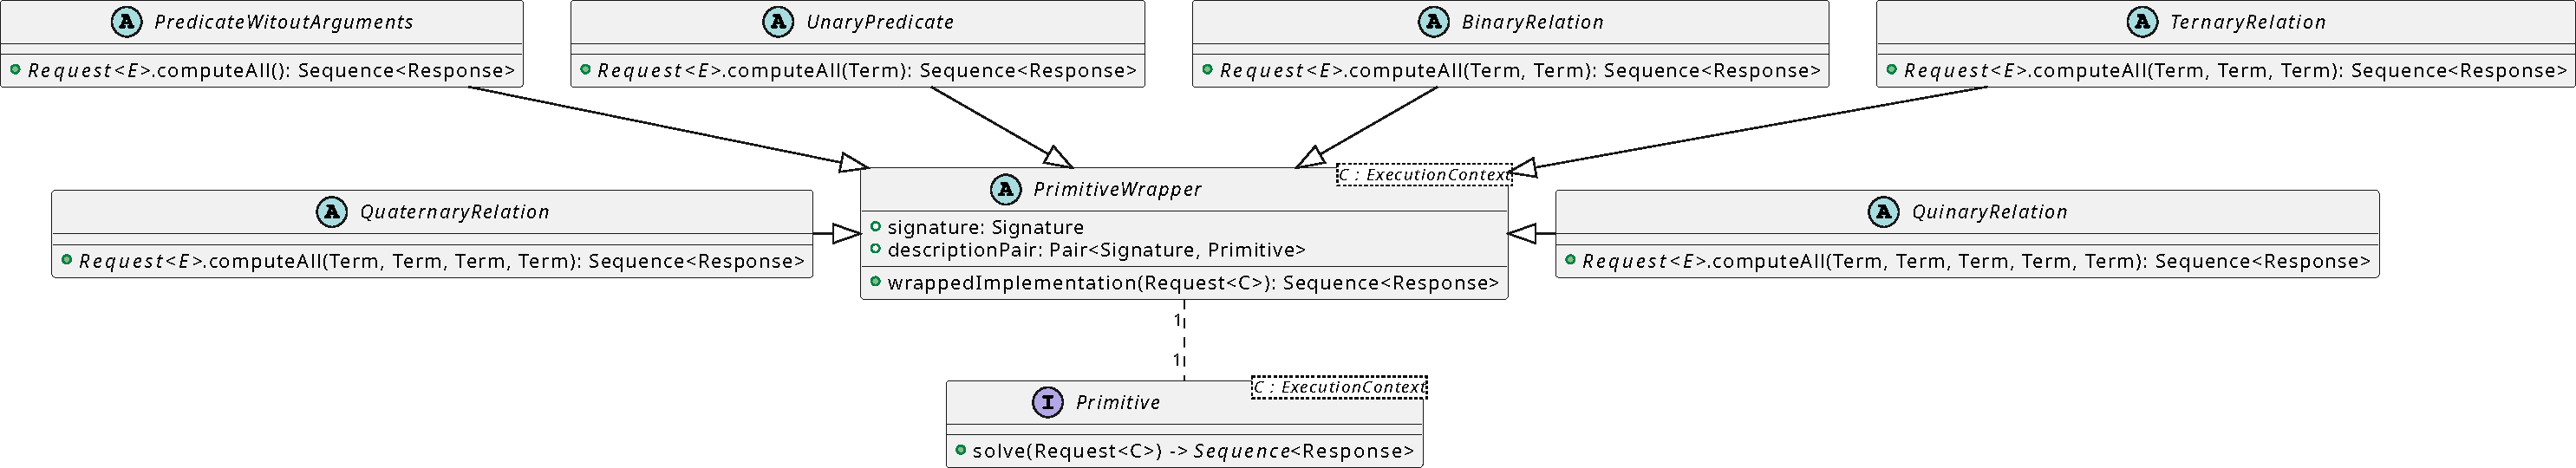
\includegraphics[width=\linewidth]{figures/wrappers.pdf}
    \end{center}

    \framebreak

    Main wrapper classes:
    %
    \begin{description}
        \item[\kt{PredicateWithoutArguments}] base class for 0-ary predicates
        \item[\kt{UnaryPredicate}] base class for 1-ary predicates
        \item[\kt{BinaryRelation}] base class for 2-ary predicates
        \item[\kt{TernaryRelation}] base class for 3-ary predicates
        \item[\kt{QuaternaryRelation}] base class for 4-ary predicates
        \item[\kt{QuinaryRelation}] base class for 5-ary predicates
    \end{description}

    \framebreak

    Each wrapper class, comes with 4 more abstract sub-classes:
    %
    \begin{description}
        \item[\kt{WithoutSideEffects}] to be preferred if the predicate does not provoke side-effects
        \item[\kt{NonBacktrackable}] to be preferred if the predicate is not backtrackable, yet it may provoke side-effects
        \item[\kt{Functional}] to be preferred if the predicate is not backtrackable and does not provoke side-effects
        \item[\kt{Predicative}] to be preferred if the predicate has a boolean semantics, i.e. it is not backtrackable, it does not provoke side-effects, and it does not assign any variable
    \end{description}
\end{frame}

\begin{frame}{\kt{PrimitiveWrapper}s in \twopkt{} -- Example: \pl{natural/1} (bis)}
    \kotlinimport[basicstyle=\tiny\ttfamily]{listings/NatPrimitive2.kt}
\end{frame}

\begin{frame}[allowframebreaks]{About \kt{PrimitiveWrapper}s' Utility Methods}\small

    Each sub-class of \kt{PrimitiveWrapper} inherits a number of protected utility methods:
    %
    \begin{description}\small
        \item[\kt{ensuringAllArgumentsAreInstantiated()}] throws an \kt{InstantiationError} if some argument is a \kt{Var}
        % \framebreak
        \item[\kt{ensuringArgumentIsWellFormedIndicator(Int)}] checks whether the argument at the provided index is a well formed indicator (i.e. \pl{\meta{Atom}/\meta{Integer}}), throwing the most adequate error in case it is not
        % \framebreak
        \item[\kt{ensuringArgumentIsWellFormedClause(Int)}] checks whether the argument at the provided index is a well formed clause (i.e. no sub-goal in the body is a \kt{Var}), throwing the most adequate error in case it is not
        % \framebreak
        \item[\kt{ensuringArgumentIsInstantiated(Int)}] throws an \kt{InstantiationError} if the argument at the provided index is a \kt{Var}
        % \framebreak
        \item[\kt{ensuringArgumentIsNumeric(Int)}] throws a \kt{TypeError} if the argument at the provided index is not \kt{Numeric}
        % \framebreak
        \item[\kt{ensuringArgumentIsStruct(Int)}] throws a \kt{TypeError} if the argument at the provided index is not a \kt{Struct}
        % \framebreak
        \item[\kt{ensuringArgumentIsCallable(Int)}] alias for \kt{ensuringArgumentIsStruct}
        % \framebreak
        \item[\kt{ensuringArgumentIsVariable(Int)}] throws a \kt{TypeError} if the argument at the provided index is not a \kt{Var}
        % \framebreak
        \item[\kt{ensuringArgumentIsCompound(Int)}] throws a \kt{TypeError} if the argument at the provided index is not a \kt{Struct} s.t. $\kt{arity} > 0$
        % \framebreak
        \item[\kt{ensuringArgumentIsAtom(Int)}] throws a \kt{TypeError} if the argument at the provided index is not an \kt{Atom}
        % \framebreak
        \item[\kt{ensuringArgumentIsConstant(Int)}] throws a \kt{TypeError} if the argument at the provided index is not a \kt{Constant}
        % \framebreak
        \item[\kt{ensuringArgumentIsGround(Int)}] throws an \kt{InstantiationError} if the argument at the provided index is not \emph{ground}
        % \framebreak
        \item[\kt{ensuringArgumentIsChar(Int)}] throws a \kt{TypeError} if the argument at the provided index is not an \kt{Atom} s.t. $\kt{value.length} == 1$
        % \framebreak
        \item[\kt{ensuringArgumentIsSpecifier(Int)}] throws a \kt{DomainError} if the argument at the provided index is not an \kt{Atom} from the set \pl{\{fx, fy, xf, yf, xfx, yfx, xfy\}}
        % \framebreak
        \item[\kt{ensuringArgumentIsList(Int)}] throws a \kt{TypeError} if the argument at the provided index is not an \kt{List}
        % \framebreak
        \item[\kt{ensuringArgumentIsInteger(Int)}] throws a \kt{TypeError} if the argument at the provided index is not an \kt{Integer}
        % \framebreak
        \item[\kt{ensuringArgumentIsNonNegativeInteger(Int)}] throws a \kt{TypeError} if the argument at the provided index is not an \kt{Integer}, or a \kt{DomainError} if it is a negative integer
        % \framebreak
        \item[\kt{ensuringArgumentIsArity(Int)}] throws a \kt{TypeError} if the argument at the provided index is not an \kt{Integer}, a \kt{DomainError} if it is a negative integer, or a \kt{RepresentationError} is it is an integer greater than \kt{MaxArity.defaultValue}
        % \framebreak
        \item[\kt{ensuringArgumentIsWellFormedList(Int)}] throws a \kt{TypeError} if the argument at the provided index is not an \kt{List}, or a \kt{DomainError} if it is a \kt{List} whose termination item is not \pl{[]}
        % \framebreak
        \item[\kt{ensuringArgumentIsCharCode(Int)}] throws a \kt{RepresentationError} if the argument at the provided index does not correspond to a character according to the UTF-16 encoding
        % \framebreak
        \item[\kt{checkTermIsRecursivelyCallable(Term)}] checks whether the provided \kt{Term} is a well formed clause (i.e. no sub-goal in the body is a \kt{Var}), throwing the most adequate error in case it is not
        % \framebreak
        \item[\kt{ensuringTermIsCharCode(Term)}] throws a \kt{RepresentationError} if the provided \kt{Term} does not correspond to a character according to the UTF-16 encoding
        % \framebreak
        \item[\kt{ensuringTermIsWellFormedList(Term)}] throws a \kt{TypeError} if the provided \kt{Term} is not an \kt{List}, or a \kt{DomainError} if it is a \kt{List} whose termination item is not \pl{[]}
        % \framebreak
        \item[\kt{ensuringProcedureHasPermission(Signature, PermissionError.Operation)}] throws a \kt{PermissionError} is the provided \kt{Signature} matches some entry among the \kt{Solver}'s libraries, or static KB
        % \framebreak
        \item[\kt{ensuringClauseProcedureHasPermission(Clause, PermissionError.Operation)}] same as above, except that the \kt{Signature} of the \kt{Clause}'s \kt{head} is considerer
    \end{description}
\end{frame}

\begin{frame}{Other Examples: \pl{assert/1}}
    \kotlinimport[basicstyle=\tiny\ttfamily]{listings/Assert.kt}
\end{frame}

\begin{frame}{Other Examples: \pl{retract/1}}
    \kotlinimport[basicstyle=\tiny\ttfamily]{listings/Retract.kt}
\end{frame}

%===============================================================================
\section{Exercises}
%===============================================================================

\begin{frame}{Exercises}
\label{slide:exercies} 

    \begin{block}{Repository}\centering
        \url{https://gitlab.com/pika-lab/courses/ise/ay2122/lab-3}
    \end{block}
    %
    \begin{itemize}
        \startExercise
        \item[] \alert{\currentExercise{}} --- Implement the \pl{read\_text/2} action as a primitive
        
        \startExercise
        \item[] \alert{\currentExercise{}} --- Implement the \pl{write\_text/2} action as a primitive
        
        \startExercise
        \item[] \alert{\currentExercise{}} --- Implement the \pl{update/1} action as a primitive
        %
        \begin{itemize}
            \item this should be equivalent to the following meta-rule:
            %
            \begin{center}
                \begin{tabular}{l}
                    \pl{update($f$($a_1$, \ldots, $a_n$)) :- }
                    \\
                    \qquad \pl{retract($f$(X$_1$, \ldots, X$_n$)),}
                    \\
                    \qquad \pl{!,}
                    \\
                    \qquad \pl{assert($f$($a_1$, \ldots, $a_n$)).}
                \end{tabular}
            \end{center}
            \item try then re-writing the agent from slide \ref{slide:achievement} using \pl{update/1}
        \end{itemize} 
    \end{itemize}
\end{frame}

%===============================================================================
\section*{}
%===============================================================================

%/////////
\frame{\titlepage}
%/////////

%===============================================================================
\section*{\refname}
%===============================================================================

%%%%
\setbeamertemplate{page number in head/foot}{}
%/////////
\begin{frame}[c,noframenumbering]{\refname}
%\begin{frame}[t,allowframebreaks,noframenumbering]{\refname}
%	\tiny
    \scriptsize
%	\footnotesize
    \bibliographystyle{apalike-AMS}
    \bibliography{ise-lab-perception-actuation}
\end{frame}
%/////////

%%%%%%%%%%%%%%%%%%%%%%%%%%%%%%%%%%%%%%%%%%%%%%%%%%%%%%%%%%%%%%%%%%%%%%%%%%%%%%%%
\end{document}
%%%%%%%%%%%%%%%%%%%%%%%%%%%%%%%%%%%%%%%%%%%%%%%%%%%%%%%%%%%%%%%%%%%%%%%%%%%%%%%%
